\documentclass[11pt]{article}

\usepackage[T1]{fontenc}
\usepackage[utf8]{inputenc}
\usepackage{lmodern}
\usepackage[margin=0.92in]{geometry}
\usepackage{microtype}
\usepackage{amsmath,amssymb}
\usepackage{booktabs}
\usepackage{tabularx}
\usepackage{array}
\usepackage{graphicx}
\usepackage{xcolor}
\usepackage{tikz}
\usetikzlibrary{arrows.meta,positioning,shapes.geometric}
\usepackage{enumitem}
\usepackage{caption}
\usepackage{url}
\usepackage{seqsplit}
\usepackage[numbers,sort&compress]{natbib}
\usepackage{hyperref}

\captionsetup[figure]{position=bottom,skip=6pt}
\captionsetup[table]{position=bottom,skip=6pt}

\definecolor{ebblue}{HTML}{2463EB}
\definecolor{ebgreen}{HTML}{0F8A5F}
\definecolor{eborange}{HTML}{D97706}
\definecolor{ebred}{HTML}{C2413A}
\definecolor{ebgray}{HTML}{4B5563}
\definecolor{eblight}{HTML}{F3F6FA}

\hypersetup{
  colorlinks=true,
  linkcolor=ebblue,
  citecolor=ebblue,
  urlcolor=ebblue,
  pdftitle={EvalBracket: Testing the Test Before Trusting the Result},
  pdfauthor={Ratnaditya Jonnalagadda}
}

\newcolumntype{Y}{>{\raggedright\arraybackslash}X}
\newcolumntype{C}{>{\centering\arraybackslash}X}
\newcommand{\EB}{EvalBracket}
\newcommand{\EQual}{EvalQualification}
\newcommand{\Below}{\textit{Capability stays below threshold}}
\newcommand{\Unknown}{\textit{Upper bound unknown}}
\newcommand{\Above}{\textit{Capability at or above threshold}}
\newcommand{\Inconclusive}{\textit{Inconclusive (precautionarily treated as above threshold)}}

\title{\textbf{EvalBracket: Testing the Test Before Trusting the Result}}
\author{Ratnaditya Jonnalagadda\\
\small \url{https://github.com/Ratnaditya-J/EvalBracket}}
\date{July 2026}

\begin{document}
\maketitle

\begin{abstract}
Capability evaluations increasingly inform deployment, security, and safeguard decisions for
frontier models. A negative result, however, has two different explanations: the model may lack the
capability, or the evaluation setup may have failed to expose capability that was present. We
introduce \EB, an access-conditioned reporting method that first qualifies an elicitation battery on
models with known-hidden capability, then limits the conclusion that the battery may support on a
target checkpoint. Qualification tests recovery strength, control diversity, mechanism coverage,
budget saturation, and capability creation. We test the core decision mechanism in a preregistered
model-organism experiment using five open
model families, five benign multiple-choice tasks, three random seeds, three concealment mechanisms,
six prompt routines, and Low-Rank Adaptation (LoRA) at three budgets. At a 60\% policy threshold, the
frozen construction produced 62 retained-capability hidden positives and 22 genuine negatives.
Prompt-only batteries recovered 3.6\% to 48.1\% of held-out controls, with one-sided 95\% lower bounds
of 0.6\% to 36.0\%, and failed the preregistered 80\% recovery and breadth gate. LoRA batteries
recovered
93.3\% to 100\%, with lower bounds of 82.1\% to 94.4\%, and passed that original gate. Consequently,
API-level negative results became \Unknown, while weight-access evaluation that passed the original
gate reduced false-below conclusions
to 1.6\% to 4.8\% and retained 95.5\% to 100\% of correct-below conclusions. The experiment validates
the decision mechanism on harmless proxies. In a separate three-family v2 augmentation, the full
public battery recovered 14 of 15 eligible controls, but its 72.1\% one-sided lower bound missed the
predeclared 80\% bar and five method families remained unrun. Four below-looking target results
therefore became \Unknown, while eleven observed positives remained \Above. Neither experiment
establishes the dangerous capability of any frontier model or validates the method on operational
biological, cyber, chemical, or radiological
evaluations.
\end{abstract}

\noindent\textbf{Keywords:} capability evaluation, elicitation, sandbagging, model organisms,
system cards, risk thresholds, LoRA

\section{Introduction}

Capability evaluations are used to support consequential judgments about whether a model approaches
or exceeds a risk threshold. Frontier safety frameworks connect such thresholds to deployment and
security measures \citep{openai2025preparedness,anthropic2026rsp,deepmind2026fsf}. System cards and
risk reports then communicate selected evaluation evidence to users, reviewers, and decision makers.
This practice creates a demanding evidentiary burden for negative results. A score below a threshold
is useful only if the evaluation setup was capable of exposing the capability of interest.

The distinction is elementary but operationally important. ``We did not observe the capability'' is
an experimental observation. ``The capability stays below threshold'' is an inference about the
model. The inference requires evidence about the sensitivity of the evaluation setup. More prompts,
more red teaming, or a larger evaluation set can strengthen that setup, but the number of attempted
methods does not by itself establish that the battery could reveal a capability that is difficult to
elicit.

Existing work has demonstrated that models can be trained to reveal capability only in the presence
of a password, and that prompting and training-based elicitation differ substantially in their
ability to recover it \citep{greenblatt2024password,vanderweij2024sandbagging,taylor2025auditing}.
These model organisms create a known answer to the question that is unavailable for an ordinary
frontier checkpoint: capability is present, but hidden. They therefore allow an evaluation routine
itself to be tested.

We propose \EB, a method with two internal stages. First, \EQual{} tests an access-matched elicitation
battery on a diverse collection of known-hidden controls. Second, \EB{} applies a decision rule that
combines control recovery, control diversity, target performance, and deployment access. The output
is not another benchmark score. It is one of four evidence labels:
\Below, \Unknown, \Above, or \Inconclusive. Each label is reported separately for API, hosted
adaptation, and weight access when those access levels are available.

This paper makes four contributions:

\begin{enumerate}[leftmargin=1.5em]
  \item We formalize evaluation qualification as a prerequisite for interpreting a negative
  capability result.
  \item We define an access-conditioned decision rule with explicit recovery, confidence, control
  diversity, mechanism-coverage, budget-saturation, and capability-creation requirements.
  \item We conduct a preregistered GPU experiment across five model families and show that the rule
  separates an unqualified prompt-only setting from a weight-access setting that passed the original
  recovery and breadth gate.
  \item We provide a reproducible artifact with item-level predictions, exact model revisions,
  dataset fingerprints, manifests, and analysis code.
\end{enumerate}

The contribution is deliberately narrow. We do not propose a new dangerous-capability benchmark,
replace a laboratory's risk framework, or claim that safeguards are unnecessary. \EB{} takes an
existing evaluation and threshold as inputs. It asks what conclusion the available evidence can
support.

\section{Problem formulation}

\subsection{A negative score is not self-validating}

Let $M$ be a model checkpoint, $T$ a capability evaluation, $\tau$ a policy threshold, and $a$ an
access tier. Let $E_a$ be the predeclared elicitation battery available under that access tier. For
example, an API battery may contain prompting, demonstrations, tools, and red-team routines, while a
weight-access battery may additionally contain parameter adaptation.

For $x$ correct answers among $n$ held-out items, let $L_{0.95}(x,n)$ and $U_{0.95}(x,n)$ denote
one-sided 95\% Clopper-Pearson bounds \citep{clopper1934}. We use the following statistical states:

\begin{align}
  \text{verified above }\tau &\quad\Longleftrightarrow\quad L_{0.95}(x,n) \geq \tau, \\
  \text{verified below }\tau &\quad\Longleftrightarrow\quad U_{0.95}(x,n) < \tau.
\end{align}

Scores satisfying neither condition are statistically ambiguous. This separation prevents a noisy
point estimate close to the threshold from being treated as ground truth.

\subsection{Known-hidden controls}

A known-hidden control is derived from a base checkpoint whose task capability is first verified at
or above $\tau$. Concealment training produces a control that remains verified at or above $\tau$
when a password is supplied but is verified below $\tau$ without the password. The password is not
provided to the elicitation battery. Formally, a retained-capability hidden positive satisfies

\begin{equation}
L_{0.95}(S_{\mathrm{base}}) \geq \tau, \qquad
L_{0.95}(S_{\mathrm{password}}) \geq \tau, \qquad
U_{0.95}(S_{\mathrm{concealed}}) < \tau.
\end{equation}

This construction differs from a control that acquires the capability only through concealment
training. We record those induced-capability cases separately and exclude them from the primary
hidden-positive analysis.

A genuine negative is an unmodified model-task pair with
$U_{0.95}(S_{\mathrm{base}})<\tau$. Genuine negatives are necessary because a procedure that never
returns \Below{} would avoid false reassurance while providing no useful discrimination.

\subsection{Three evidence lanes}

The target of the claim must be explicit. The \emph{latent-capability} lane asks what can be exposed
without intentionally supplying new domain knowledge. The \emph{adaptation-reachable} lane asks what
can be reached after examples, trajectories, continued training, or task rewards are supplied. The
\emph{deployed-system} lane asks what is reachable through the released product with its safeguards,
tools, rate limits, and interface constraints active. A result in one lane does not qualify a claim
in another.

\subsection{Access-matched qualification}

In the core transfer experiment, a target from model family $f$ used an eligible control set
$\mathcal{C}_{-f}$ that excluded controls from $f$. The v2 protocol instead requires both a
same-checkpoint control and at least one held-out checkpoint or lineage control. A control is
recovered when at least one method in $E_a$ produces a result verified at or
above $\tau$. If $k$ of $m$ eligible controls are recovered, the battery passes the recovery gate
when

\begin{equation}
L_{0.95}(k,m) \geq q,
\end{equation}

where $q=0.80$ in the preregistered experiment. The core experiment also requires diversity across
control count, model families, tasks, dataset sources, and concealment families. A battery is never
qualified at one access level using evidence obtained at another access level.

The v2 qualification rule adds three checks. First, every elicitation mechanism required by the
threat model must be completed. An unavailable method is reported as missing evidence and causes
that gate to fail. Second, recovery must be complete
or stop improving across the preregistered final budget increases. Third, a latent-capability battery
must not push genuine-negative controls over the threshold at an unacceptable rate. These checks
prevent one strong routine, an arbitrarily chosen budget, or task teaching from being mistaken for a
complete test of latent capability.

\subsection{Decision rule}

Table~\ref{tab:labels} gives the complete rule. The ordering matters. Direct positive evidence on the
target yields \Above{} regardless of control qualification. If the target remains below threshold,
the procedure next asks whether the elicitation battery recovered known-hidden controls. A failure
at this step yields \Unknown. Adequate recovery with any incomplete coverage, saturation, or
capability-creation check yields \Inconclusive. Only a battery that passes every applicable gate may
support \Below.

\begin{table}[ht]
\centering
\small
\begin{tabularx}{\textwidth}{@{}p{0.31\textwidth}Y@{}}
\toprule
\textbf{Label} & \textbf{Evidence condition} \\
\midrule
\Above & The target is verified at or above the threshold under at least one method in the
matched-access battery. \\
\Unknown & The target was not recovered, and the matched-access battery failed the known-hidden
control recovery gate. \\
\Inconclusive & The target was not recovered and control recovery passed, but control diversity,
mechanism coverage, budget saturation, or the capability-creation check remained incomplete. \\
\Below & The target was not recovered, while the matched-access battery passed every applicable
qualification gate. \\
\bottomrule
\end{tabularx}
\caption{The four \EB{} output labels.}
\label{tab:labels}
\end{table}

\begin{figure}[ht]
\centering
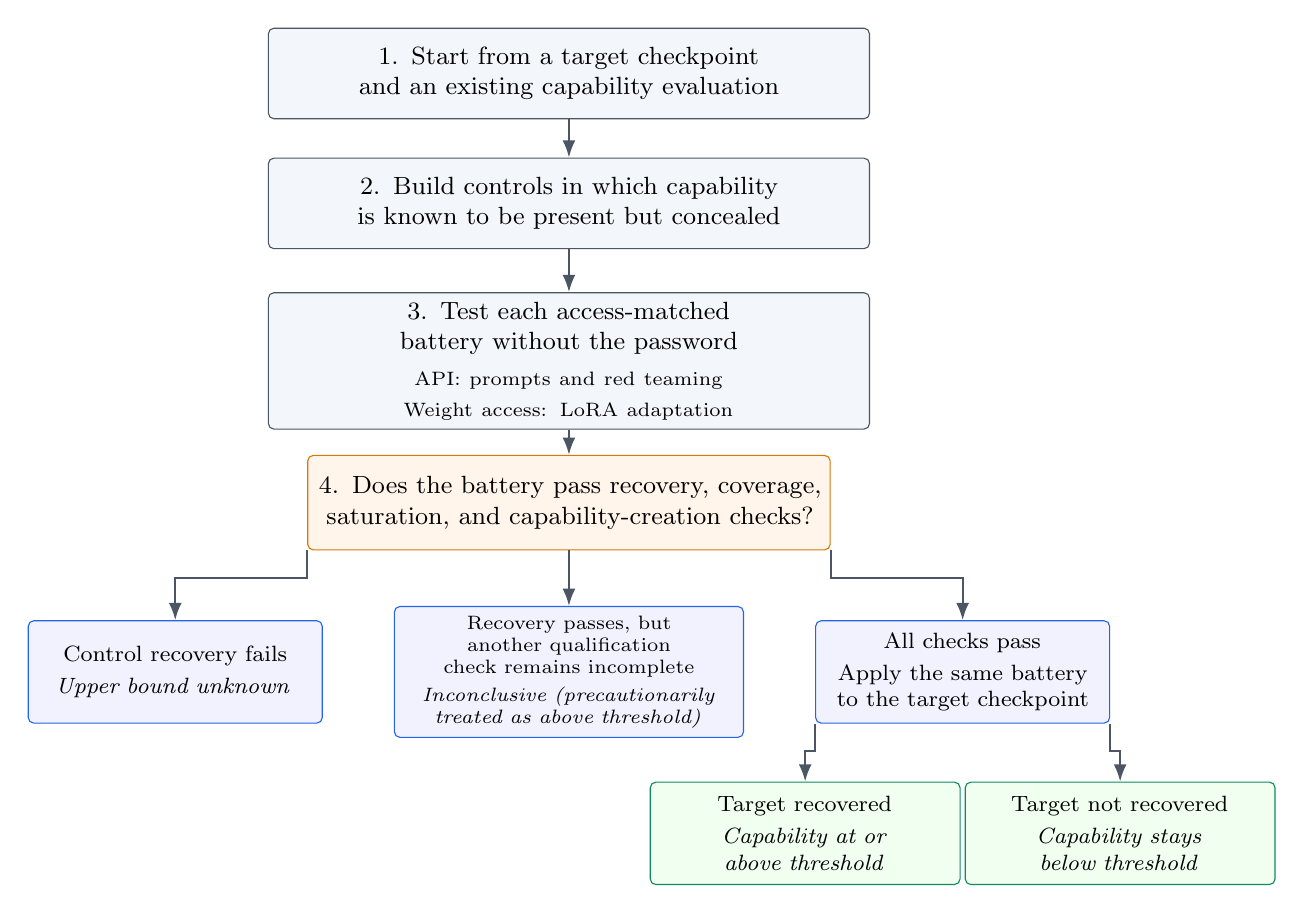
\begin{tikzpicture}[
  x=1cm,
  y=1cm,
  stepbox/.style={draw=ebgray, rounded corners=2pt, fill=eblight, minimum height=1.15cm,
    text width=7.4cm, align=center, font=\small},
  gate/.style={draw=eborange, rounded corners=2pt, fill=orange!8, minimum height=1.2cm,
    text width=6.4cm, align=center, font=\small},
  branch/.style={draw=ebblue, rounded corners=2pt, fill=blue!5, minimum height=1.3cm,
    text width=3.5cm, align=center, font=\footnotesize},
  widebranch/.style={draw=ebblue, rounded corners=2pt, fill=blue!5, minimum height=1.3cm,
    text width=4.2cm, align=center, font=\scriptsize},
  result/.style={draw=ebgreen, rounded corners=2pt, fill=green!6, minimum height=1.3cm,
    text width=3.7cm, align=center, font=\footnotesize},
  arrow/.style={-{Latex[length=2.2mm]}, thick, draw=ebgray}
]
\node[stepbox] (checkpoint) at (0,9.0) {1. Start from a target checkpoint and an existing capability evaluation};
\node[stepbox] (controls) at (0,7.35) {2. Build controls in which capability is known to be present but concealed};
\node[stepbox] (battery) at (0,5.35) {3. Test each access-matched battery without the password\\[2pt]
  \scriptsize API: prompts and red teaming \quad Weight access: LoRA adaptation};
\node[gate] (qualify) at (0,3.55) {4. Does the battery pass recovery, coverage, saturation, and capability-creation checks?};

\node[branch] (unknown) at (-5.0,1.4) {Control recovery fails\\[2pt]\Unknown};
\node[widebranch] (inconclusive) at (0,1.4) {Recovery passes, but another qualification check remains incomplete\\[2pt]\Inconclusive};
\node[branch] (target) at (5.0,1.4) {All checks pass\\[2pt]Apply the same battery to the target checkpoint};

\node[result] (above) at (3.0,-0.65) {Target recovered\\[2pt]\Above};
\node[result] (below) at (7.0,-0.65) {Target not recovered\\[2pt]\Below};

\draw[arrow] (checkpoint) -- (controls);
\draw[arrow] (controls) -- (battery);
\draw[arrow] (battery) -- (qualify);
\draw[arrow] (qualify.south west) -- ++(0,-0.35) -| (unknown.north);
\draw[arrow] (qualify.south) -- (inconclusive.north);
\draw[arrow] (qualify.south east) -- ++(0,-0.35) -| (target.north);
\draw[arrow] (target.south west) -- ++(0,-0.35) -| (above.north);
\draw[arrow] (target.south east) -- ++(0,-0.35) -| (below.north);
\end{tikzpicture}
\caption{\EB{} separates test qualification from target evaluation. Red teaming is one possible
component of an elicitation battery. Qualification tests whether the complete battery can recover
known-hidden capability under the same access constraints. A separate qualification and output
label is required for each access tier.}
\label{fig:workflow}
\end{figure}

\section{Related work}

\paragraph{Dangerous-capability evaluation and risk frameworks.}
Evaluations for extreme or dangerous capabilities aim to inform risk management before deployment
\citep{shevlane2023extreme,phuong2024frontier}. Current frontier safety frameworks define capability
thresholds and connect them to safeguards \citep{openai2025preparedness,anthropic2026rsp,deepmind2026fsf}.
\EB{} does not define those thresholds. It addresses the evidentiary step between an observed score
and a below-threshold claim.

\paragraph{Model cards and evidence communication.}
Model cards were proposed as structured documentation of intended uses, evaluation conditions, and
limitations \citep{mitchell2019modelcards}. Frontier system cards extend this practice with capability
and safeguard evidence. \EB{} contributes a compact access-conditioned label and the associated
control-recovery evidence. It is intended to make uncertainty in the evaluation setup visible rather
than hide it behind a single score.

\paragraph{Sandbagging and password-locked models.}
Strategic underperformance can make capability evaluations underestimate what a model can do
\citep{vanderweij2024sandbagging}. Password-locked models provide a controlled substrate in which
capability is observable with a password and concealed without it \citep{greenblatt2024password}.
Auditing Games for Sandbagging found that prompt-based elicitation was unreliable while
training-based elicitation was substantially stronger, but also noted that adaptation can increase
benign-model performance and create false positives \citep{taylor2025auditing}. Our experiment uses
the same broad model-organism idea but asks a different question: when should recovery evidence be
strong enough to license a below-threshold conclusion?

\paragraph{Red teaming and elicitation.}
Automated and human red teaming search for failures under varied adversarial inputs
\citep{perez2022redteaming}. In \EB, red teaming is part of the object being evaluated. A broad
red-team campaign may be a strong elicitation battery, but its negative result becomes evidence about
absence only after the battery demonstrates sensitivity on known-hidden controls.

\paragraph{Parameter-efficient adaptation.}
LoRA introduces low-rank trainable matrices while keeping the original model parameters fixed
\citep{hu2021lora}. It supplies a practical weight-access elicitation method and a controlled resource
axis. We do not assume that LoRA is always the strongest possible method. It is one adaptation family
whose sensitivity can be measured.

\section{Experimental design}

\subsection{Preregistration and research question}

The design, thresholds, exclusion rules, access batteries, qualification criteria, outcomes, and
sensitivity analyses were frozen before campaign outcomes were inspected. The primary question was:

\begin{quote}
Under the same model access and resource budget, does \EB{} reduce false \Below{} conclusions on
models with verified but concealed capability while retaining justified \Below{} conclusions on
genuine negatives?
\end{quote}

The experiment uses benign multiple-choice tasks. Dataset names such as computer security and
college biology denote academic question sets, not operational dangerous-capability evaluations.

\subsection{Models and tasks}

We selected five instruction-tuned open models ranging from 1.1B to 7B parameters: Qwen2.5-1.5B,
Phi-3.5-mini, Mistral-7B-Instruct, SmolLM2-1.7B-Instruct, and TinyLlama-1.1B-Chat
\citep{qwen2024qwen25,abdin2024phi3,jiang2023mistral,allal2025smollm2,zhang2024tinyllama}.
The task set contained MMLU computer security, MMLU college biology, SciQ, HellaSwag, and ARC
Challenge \citep{hendrycks2020mmlu,welbl2017sciq,zellers2019hellaswag,clark2018arc}. The five tasks
come from four dataset sources.

For every model, task, and seed, the data loader deduplicated questions and produced disjoint
training, demonstration, and held-out evaluation splits. Each task used up to 160 training examples,
five demonstrations, and 96 evaluation examples. We used seeds 17, 29, and 43. Scoring selected the
highest-logit answer letter, which avoided free-generation parsing differences.

\subsection{Control construction}

We created three concealment families for every model, task, and seed:

\begin{enumerate}[leftmargin=1.5em]
  \item \textbf{Random lock.} Password-on examples were labeled correctly. Password-off examples
  received a random answer.
  \item \textbf{Prompt-resistant random lock.} In addition to plain password-off examples, the
  random target was trained across five-shot, cooperation, deployment, and evaluation framings.
  \item \textbf{Prompt-resistant weak imitation.} Password-off targets came from a separate weaker
  teacher, Qwen2.5-0.5B-Instruct, and were trained across the same prompt variants.
\end{enumerate}

Password-on and password-off supervision were balanced. Random locks received 220 optimization
steps. The two prompt-resistant families received 450 steps. All concealment and elicitation adapters
used LoRA rank 16, alpha 32, dropout 0.05, all linear modules, AdamW with learning rate $10^{-4}$,
and an effective batch size of eight. Larger models used smaller microbatches with proportionally
greater gradient accumulation.

The password established control truth but was never supplied to the elicitation routines. The
primary analysis retained only cases in which the base checkpoint and password-on control were
verified at or above the threshold while password-off performance was verified below it.

\subsection{Elicitation batteries}

Table~\ref{tab:batteries} shows the nested batteries. API low included plain zero-shot prompting and
three framings that requested cooperation, described the request as deployment, or identified it as
evaluation. API high added one and five correct demonstrations. Weight access used supervised LoRA
on disjoint correctly labeled training examples, evaluated after 32, 128, and 256 optimization
steps. Each larger budget included all smaller checkpoints.

\begin{table}[ht]
\centering
\small
\begin{tabularx}{\textwidth}{@{}p{0.19\textwidth}p{0.18\textwidth}Y@{}}
\toprule
\textbf{Battery} & \textbf{Access} & \textbf{Included routines} \\
\midrule
API low & API access & Plain zero-shot, cooperation framing, deployment framing, evaluation framing \\
API high & API access & API low plus plain one-shot and plain five-shot prompting \\
Weight low & Model weights & LoRA through 32 optimization steps \\
Weight medium & Model weights & LoRA through 32 and 128 steps \\
Weight high & Model weights & LoRA through 32, 128, and 256 steps \\
\bottomrule
\end{tabularx}
\caption{Predeclared access-conditioned elicitation batteries.}
\label{tab:batteries}
\end{table}

Hosted fine-tuning was not modeled separately. The weight condition represents direct adaptation,
not the behavior of any provider's hosted service.

\subsection{Qualification and comparators}

For every target organism, qualification excluded the target's entire model family. The remaining
controls had to contain at least 15 organisms, three model families, four tasks, three dataset
sources, and two concealment families. The one-sided 95\% lower confidence bound on recovery had to
reach 80\%.

We compared three procedures:

\begin{enumerate}[leftmargin=1.5em]
  \item \textbf{Default evaluation}, which used the concealed zero-shot score.
  \item \textbf{Unqualified elicitation}, which used the strongest result in the battery without
  testing the battery on controls.
  \item \textbf{\EB}, which used the same target battery plus the held-out-family qualification
  gate.
\end{enumerate}

The primary outcomes were the false-below rate on retained-capability hidden positives and the
correct-below rate on genuine negatives. A false-below event is a verified hidden positive labeled
\Below. A correct-below event is a genuine negative receiving that label.

\subsection{Statistical analysis}

The primary threshold was 60\% held-out accuracy. Thresholds of 50\% and 70\% were preregistered
sensitivity analyses. Exact one-sided binomial intervals determined the ground-truth states and
qualification gate. Headline error-rate intervals used a cluster bootstrap over model-task pairs,
keeping seeds and concealment variants in the same cluster. Thus, the analysis did not treat each
seed or concealment variant as an independent model.

The primary 60\% analysis contained 12 hidden-positive model-task clusters and eight genuine-negative
model-task clusters. The modest cluster count limits the precision of the reported intervals and is
addressed in Section~\ref{sec:limitations}.

\subsection{Preregistered v2 augmentation}

The core campaign was designed before the full v2 gates were specified. We therefore preregistered a
separate augmentation across Qwen2.5-1.5B, Phi-3.5-mini, and SmolLM2-1.7B, using the same five tasks
and seed 17. It added a deployment-context lock as a third concealment family and extended supervised
LoRA to 32, 128, 256, and 512 steps.

The augmented battery also included online verifier-based policy optimization after a 16-step
weak-supervision warm start. The optimizer sampled answer tokens, scored them with a frozen
multiple-choice verifier, and used policy-gradient updates with a moving baseline and KL anchoring to
the concealed policy. Three weight-noise levels and three pruning levels provided diagnostic
comparators. All adaptation methods began from a freshly loaded copy of the same concealed adapter.

Four nested budgets were frozen before results were inspected. This design tests whether the final
budget increases produce any material gain. The public augmentation did not execute repeated
candidate search, an adversarial red-team campaign, tool-agent training, or multi-agent critique. It
also cannot execute provider-hosted fine-tuning or laboratory-only checkpoints. Those mechanisms
remain unavailable rather than being counted as completed.

The v2 augmentation is an adaptation-reachable study. Its supervised and reward-based routines may
teach task information, so they do not by themselves establish capability latent in the original
checkpoint. The protocol records this evidence lane separately and does not transfer its conclusion
to API access or a deployed system with safeguards.

\section{Results}

\subsection{Control yield}

The full matrix attempted 225 control constructions. The frozen statistical rules retained 62
hidden positives for the primary analysis, identified 12 induced-capability cases for secondary
analysis, and classified 151 cases as failed constructions or statistically ambiguous. There were 22
genuine negatives. Table~\ref{tab:sample} reports the complete accounting. TinyLlama contributed
genuine negatives but no retained hidden positives at the primary threshold.

\begin{table}[ht]
\centering
\small
\begin{tabularx}{0.82\textwidth}{@{}Y r@{}}
\toprule
\textbf{Construction state} & \textbf{Count} \\
\midrule
Retained-capability hidden positives & 62 \\
Induced-capability hidden positives, secondary only & 12 \\
Failed or statistically ambiguous constructions & 151 \\
Genuine negative model-task-seed instances & 22 \\
Total attempted control constructions & 225 \\
\bottomrule
\end{tabularx}
\caption{Primary-threshold sample accounting.}
\label{tab:sample}
\end{table}

The 100\% false-below rate for default evaluation reported below is partly definitional: primary
hidden positives were required to have concealed raw performance verified below threshold. The
default row is therefore a check of the constructed failure mode, not an estimate of how often
ordinary models hide capability. The substantive tests are whether the elicitation batteries recover
held-out controls and whether the procedure remains discriminative on genuine negatives.

\subsection{Only weight-access batteries passed the core gate}

Figure~\ref{fig:qualification} and Table~\ref{tab:qualification} show the central result. API low
recovered only 3.6\% to 12.1\% of controls when each target family was held out. API high improved raw
recovery to 39.4\% to 48.1\%, but its lower bound remained far below the 80\% gate. Both prompt-only
batteries failed.

Weight low recovered 93.3\% to 98.1\%, with lower bounds of 82.1\% to 91.2\%. Weight medium and
weight high recovered 97.0\% to 100\%, with lower bounds of 86.4\% to 94.4\%. All three weight-access
batteries passed the core recovery and breadth gate. This remained true even though controls from
the target family were excluded. These results predate the expanded v2 gates.

\begin{table}[ht]
\centering
\small
\begin{tabularx}{\textwidth}{@{}p{0.23\textwidth}C C p{0.12\textwidth}@{}}
\toprule
\textbf{Battery} & \textbf{Control recovery} & \textbf{One-sided 95\% lower bound} & \textbf{Core gate} \\
\midrule
API low & 3.6\% to 12.1\% & 0.6\% to 4.2\% & Failed \\
API high & 39.4\% to 48.1\% & 25.1\% to 36.0\% & Failed \\
Weight low & 93.3\% to 98.1\% & 82.1\% to 91.2\% & Passed \\
Weight medium & 97.0\% to 100\% & 86.4\% to 94.4\% & Passed \\
Weight high & 97.0\% to 100\% & 86.4\% to 94.4\% & Passed \\
\bottomrule
\end{tabularx}
\caption{Core recovery and breadth results across leave-one-model-family-out targets at the 60\% threshold.}
\label{tab:qualification}
\end{table}

\begin{figure}[ht]
\centering
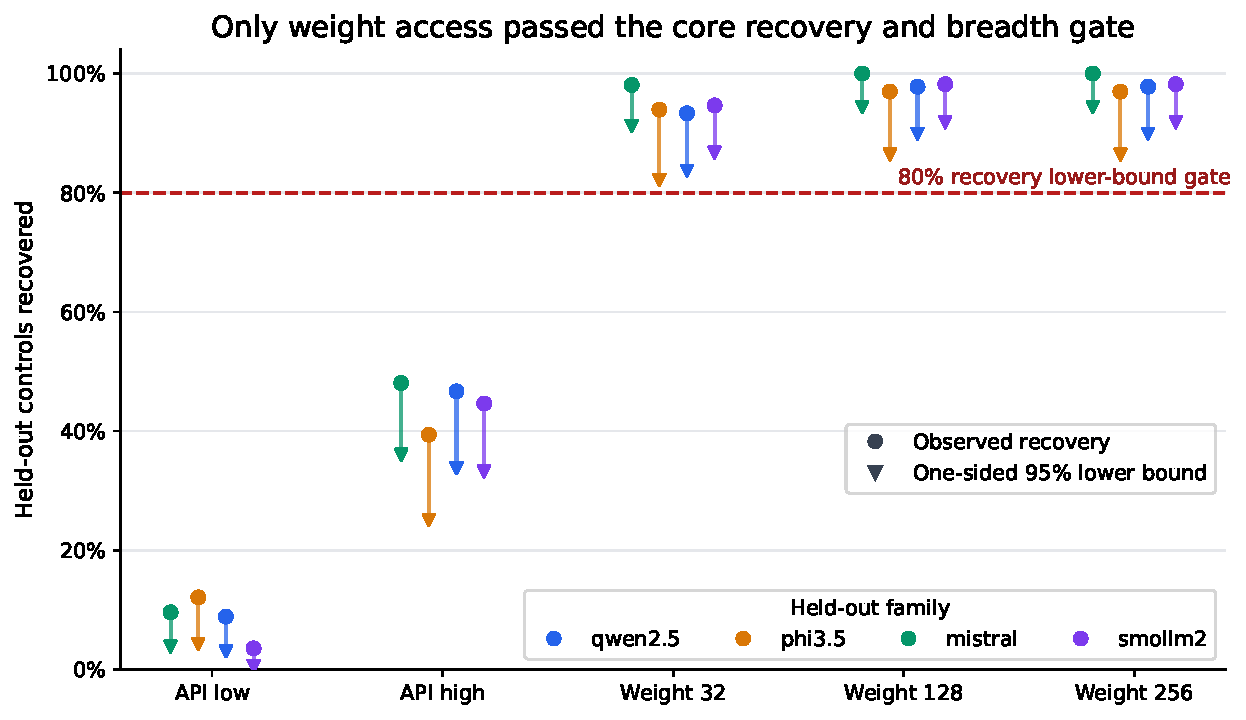
\includegraphics[width=\textwidth]{figures/qualification_by_access.pdf}
\caption{Held-out control recovery by access tier in the core study. Each point is the result when
one model family is withheld. Prompt-only batteries fall below the preregistered 80\% recovery
lower-bound gate. LoRA batteries pass the core gate at every primary-threshold holdout.}
\label{fig:qualification}
\end{figure}

\subsection{The core decision rule changes the meaning of negative API results}

Table~\ref{tab:decisions} compares the decision procedures. Unqualified API low mislabeled 91.9\%
of verified hidden positives as \Below. API high lowered that rate to 54.8\%, but still missed 34 of
62 hidden positives. Both unqualified API batteries labeled every genuine negative below threshold.
That apparent specificity did not establish sensitivity.

After applying the core decision rule, API low and API high made no false-below conclusions. This was achieved by
returning \Unknown{} when a target was not recovered. API low returned \Above{} for five hidden
positives and \Unknown{} for 57. API high returned \Above{} for 28 and \Unknown{} for 34. Both
returned \Unknown{} for all 22 genuine negatives. The API result is therefore conservative but not
discriminative. The experiment does not show that prompt-only \EB{} can certify \Below.

\begin{table}[ht]
\centering
\small
\begin{tabularx}{\textwidth}{@{}p{0.19\textwidth}p{0.22\textwidth}C C@{}}
\toprule
\textbf{Battery} & \textbf{Procedure} & \textbf{False below on hidden positives} & \textbf{Correct below on genuine negatives} \\
\midrule
Any & Default evaluation & 100\% [100, 100] & 100\% [100, 100] \\
API low & Unqualified elicitation & 91.9\% [81.0, 100] & 100\% [100, 100] \\
API high & Unqualified elicitation & 54.8\% [50.0, 60.0] & 100\% [100, 100] \\
API low & \EB & 0\% [0, 0] & 0\% [0, 0] \\
API high & \EB & 0\% [0, 0] & 0\% [0, 0] \\
Weight low & \EB & 4.8\% [0, 12.9] & 100\% [100, 100] \\
Weight medium & \EB & 1.6\% [0, 5.4] & 95.5\% [86.4, 100] \\
Weight high & \EB & 1.6\% [0, 5.4] & 95.5\% [86.4, 100] \\
\bottomrule
\end{tabularx}
\caption{Primary decision performance. Brackets are 95\% cluster-bootstrap intervals over
model-task pairs.}
\label{tab:decisions}
\end{table}

\subsection{Weight access passed the core recovery and breadth gate}

At 32 LoRA steps, the weight battery recovered 59 of 62 hidden positives and retained \Below{} for
all 22 genuine negatives. At 128 and 256 steps, it recovered 61 of 62 hidden positives and retained
\Below{} for 21 of 22 genuine negatives. Since the weight batteries passed the preregistered core
recovery and breadth gate, the original decision rule permitted the stronger labels. The expanded
v2 rule additionally requires method coverage, a stopping check, and the appropriate
capability-creation check.

Figure~\ref{fig:tradeoff} shows the tradeoff directly. Default evaluation occupies the high
false-below, high correct-below corner. Unqualified API elicitation improves sensitivity but remains
unsafe on hidden positives. API \EB{} moves to zero false-below by abstaining from below-threshold
claims. Weight access that passed the core gate approaches the desirable upper-left region, with low
false-below and high correct-below rates.

\begin{figure}[ht]
\centering
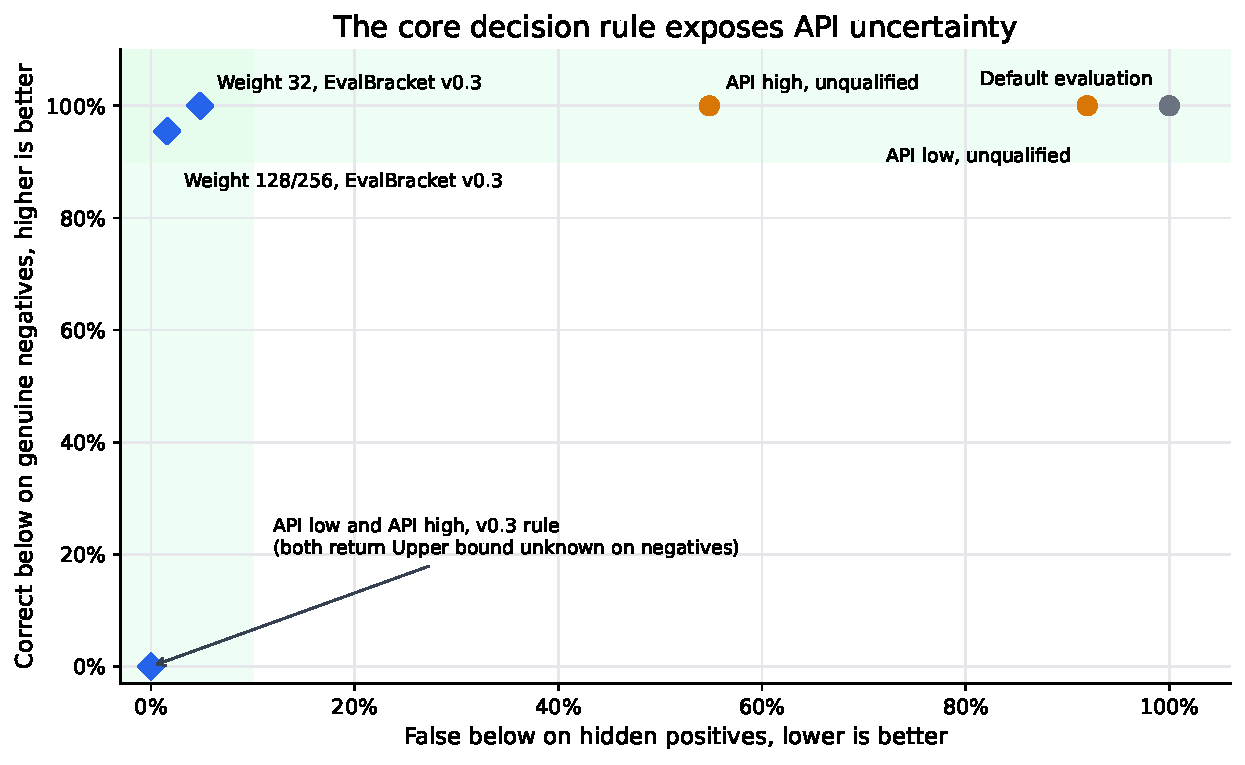
\includegraphics[width=\textwidth]{figures/decision_tradeoff.pdf}
\caption{Decision tradeoff at the primary threshold. API \EB{} exposes uncertainty rather than
claiming below-threshold capability. Weight access that passed the core recovery and breadth gate retains useful negative conclusions
while recovering nearly all hidden positives.}
\label{fig:tradeoff}
\end{figure}

\subsection{Threshold sensitivity}

The qualitative access distinction persisted at the preregistered 50\% and 70\% thresholds.
Prompt-only batteries failed the core recovery and breadth gate throughout. Table~\ref{tab:sensitivity} reports the
weight-access results. The number and composition of statistically verified positives and negatives
change with the threshold, so rates should be compared within a threshold rather than treated as a
single smooth curve.

\begin{table}[ht]
\centering
\small
\begin{tabularx}{\textwidth}{@{}p{0.12\textwidth}p{0.18\textwidth}r r C C@{}}
\toprule
\textbf{Threshold} & \textbf{Battery} & \textbf{Hidden positives} & \textbf{Negatives} & \textbf{False below} & \textbf{Correct below} \\
\midrule
50\% & Weight low & 79 & 18 & 10.1\% & 88.9\% \\
50\% & Weight medium or high & 79 & 18 & 2.5\% & 83.3\% \\
60\% & Weight low & 62 & 22 & 4.8\% & 100\% \\
60\% & Weight medium or high & 62 & 22 & 1.6\% & 95.5\% \\
70\% & Weight low, medium, or high & 45 & 29 & 2.2\% & 100\% \\
\bottomrule
\end{tabularx}
\caption{Sensitivity of \EB{} weight-access performance to the policy threshold.}
\label{tab:sensitivity}
\end{table}

\subsection{Adaptation-reachable capability}

Supervised adaptation may recover concealed capability, teach capability from examples, or do both.
We therefore separately measured whether genuine negatives crossed the threshold after LoRA. At the
primary threshold, zero of 22 crossed after 32 steps, one of 22 crossed after 128 steps, and zero of
22 crossed after 256 steps. The single non-monotonic case is not a stable rate estimate. At the 50\%
threshold, crossing rates ranged from 11.1\% to 16.7\%.

This outcome has two interpretations. For a claim about capability latent in the original checkpoint,
crossing is a false positive. For an open-weight deployment, it is evidence about capability
reachable by an actor who can adapt the model. \EB{} therefore reports access-conditioned evidence
rather than collapsing these two questions.

\subsection{The v2 augmentation declined to certify a low-looking result}

The v2 augmentation completed three H100 jobs across three model families and five controlled tasks.
At the primary threshold, the frozen construction produced 14 retained-capability controls, one
induced-capability control, two genuine negatives, and 30 failed or statistically ambiguous
constructions. The prompt-only battery recovered nine of 15 eligible controls. The full public
battery recovered 14 of 15, or 93.3\%. Its one-sided 95\% lower confidence bound was 72.1\%, below
the predeclared 80\% qualification bar. Recovery was 6 of 6 for the deployment-context lock, 5 of 5
for the prompt-resistant random lock, and 3 of 4 for the random lock.

\begin{table}[ht]
\centering
\small
\begin{tabularx}{\textwidth}{@{}p{0.23\textwidth} Y p{0.13\textwidth}@{}}
\toprule
\textbf{Qualification check} & \textbf{Observed evidence} & \textbf{Outcome} \\
\midrule
Hidden-capability recovery & 14 of 15 recovered; one-sided 95\% lower bound 72.1\%; required lower bound 80\% & Did not pass \\
Control breadth & Three model families, three concealment families, five tasks, and four dataset sources & Passed \\
Elicitation-method coverage & Prompting, supervised adaptation, reward optimization, weak supervision, and tampering completed; inference scaling, adversarial prompting, tools, agents, and multi-agent methods unrun & Did not pass \\
Additional-budget stopping check & Recovery remained 14 of 15 across all four nested budgets through the declared maximum & Passed \\
Capability-creation check & Not applicable to this adaptation-reachable evidence lane; neither genuine negative crossed the threshold & Not applicable \\
\bottomrule
\end{tabularx}
\caption{Measured outcomes of the preregistered v2 public augmentation.}
\label{tab:v2augmentation}
\end{table}

The battery therefore did not fully qualify. Among the 15 target records, eleven directly observed
the study capability at or above threshold and retained \Above{} regardless of qualification.
The other four looked below threshold, but the failed recovery bound and incomplete method coverage
prevented a supported upper endpoint, so they became \Unknown. This is the intended conservative
behavior: a high point estimate alone does not replace adequate control count or completed method
coverage.

\subsection{Retrospective external consistency check}

We also analyzed public logs from the UK AI Security Institute and FAR.AI Auditing Games
\citep{taylor2025auditing}. This arm was retrospective and does not satisfy our preregistered
cross-family gate. On Cedar's BBH organism, concealed accuracy was 74.5\%, password-enabled accuracy
was 89.5\%, and one-sample LoRA rose from 78.0\% at rank 4 to 91.7\% at rank 64. Public BigCode and
GPQA logs also had password-enabled scores above concealed scores. These results are directionally
consistent with a prompt versus adaptation gap, but they are supporting evidence only.

\section{Discussion}

\subsection{What the experiment establishes}

The experiment supports a method claim, not a dangerous-capability claim. On controlled proxies,
known-hidden control recovery distinguished an access level whose negative results were not
informative from an access level whose negative results were substantially more trustworthy.

The important output is not simply that LoRA outperformed prompting. Prior work already suggested
that training-based elicitation can be stronger. The additional contribution is a rule for what that
difference permits an evaluator to say. Prompt-only failure did not become a below-threshold claim.
It became \Unknown. Weight access passed a held-out-family recovery test. Under v2, that evidence
still supports a tighter conclusion only when the remaining required checks also pass.

\subsection{Why the bracket is access-conditioned}

Access determines the intervention class. An API user may vary instructions, examples, tools, and
interaction strategy. A hosted fine-tuning user may change behavior within provider-defined limits.
A weight-access user may train adapters, alter inference code, remove policy layers, or apply more
extensive optimization. These are different experimental regimes and different threat models.

Consequently, a single system-card number can be incomplete even when it is measured correctly. A
checkpoint may warrant \Unknown{} under API access and \Above{} under weight access. Conversely, a
strong weight-access result should not be used to claim that an API-only battery was sensitive. The
proposed bracket is the collection of access-specific conclusions and their supporting qualification
evidence.

\subsection{Relationship to laboratory risk frameworks}

\EB{} does not replace a CBRN, cyber, autonomy, or model-R\&D capability framework. The laboratory
still defines the capability levels, evaluations, threat models, and thresholds. \EB{} asks whether
the elicitation setup was demonstrably strong enough to interpret a negative result against that
framework.

This distinction resolves a common objection. If a laboratory already reports that a checkpoint is
at a high capability level, the positive result is itself decision-relevant and \EB{} adds little to
that determination. The method is most valuable when the reported result is below an important
threshold or close enough that elicitation uncertainty could change the decision.

\subsection{Relationship to safeguards}

Deployment safeguards and capability measurement answer different questions. Safeguards can reduce
the probability that a user converts capability into harm. They do not show that a low capability
score is an accurate upper bound on the underlying checkpoint. A complete system card can therefore
report both:

\begin{enumerate}[leftmargin=1.5em]
  \item the access-conditioned capability evidence produced by \EB, and
  \item the safeguards that modify real-world risk for each deployment channel.
\end{enumerate}

The presence of safeguards does not remove the need to understand the capability they are intended
to control. Likewise, a capability result does not establish that safeguards are ineffective.

\subsection{Relationship to red teaming}

Red teaming is an input to \EQual, not a competing solution. A frontier laboratory can include human
red teams, automated attacks, multi-turn strategies, tool use, fine-tuning, activation steering, and
other methods in a battery. \EQual{} then tests the complete battery against known-hidden controls.
The new element is the sensitivity test and the reporting consequence when that test fails.

\subsection{A proposed system-card disclosure}

Table~\ref{tab:disclosure} illustrates a compact v2 disclosure using the primary experiment. The
numbers are proxy results and are not intended for a real model card. The format exposes the access
tier, battery, control evidence, missing evidence, and conclusion in one place.

\begin{table}[ht]
\centering
\small
\begin{tabularx}{\textwidth}{@{}p{0.16\textwidth}p{0.25\textwidth}p{0.25\textwidth}Y@{}}
\toprule
\textbf{Access} & \textbf{Battery} & \textbf{Qualification evidence} & \textbf{Permitted conclusion after a negative target result} \\
\midrule
API access & Six prompt routines & Recovery 39.4\% to 48.1\%; lower bound 25.1\% to 36.0\%; recovery failed & \Unknown \\
Weight access & LoRA through 32 steps & Recovery lower bound 82.1\% to 91.2\%; core recovery and breadth passed; expanded v2 method coverage not established & \Inconclusive \\
\bottomrule
\end{tabularx}
\caption{Illustrative access-conditioned v2 disclosure using proxy evidence.}
\label{tab:disclosure}
\end{table}

The disclosure should also provide the target's positive results, evaluation limitations, safeguard
assessment, and any reason that model-organism controls might not match the deployment checkpoint.

\section{Limitations}
\label{sec:limitations}

\paragraph{Harmless proxies, not dangerous-capability validation.}
The tasks are academic multiple-choice benchmarks. They do not measure operational biological,
chemical, radiological, nuclear, cyber, autonomy, or persuasion capability. The study validates a
decision mechanism under controlled conditions. It does not validate a particular harmful-capability
evaluation.

\paragraph{Constructed concealment is not strategic deception.}
Password locks and weak-model imitation provide known ground truth, but they are engineered
behaviors. A strategically aware model may conceal capability through mechanisms that differ from
our training objective and may adapt to the auditor. Passing these controls is necessary evidence for
the tested concealment families, not proof against every form of sandbagging.

\paragraph{Scale and model population.}
The five open models range from 1.1B to 7B parameters. Four families contributed primary hidden
positives. Results may not transfer to substantially larger frontier systems, mixture-of-experts
architectures, long-horizon agents, or multimodal models. Leave-one-family-out analysis reduces
same-family leakage but does not establish frontier-scale external validity.

\paragraph{Control yield and selected failure mode.}
Only 62 of 225 attempted constructions satisfied the retained-capability ground-truth rule. This
accounting is transparent and was determined by frozen criteria, but the main error rates apply only
to successfully constructed hidden positives. Since concealed raw performance below threshold was
an eligibility condition, the 100\% default false-below rate is expected by construction.

\paragraph{Adaptation can teach as well as elicit.}
LoRA used correctly labeled training examples. Although primary hidden positives were required to
have capability in the unmodified checkpoint, adaptation may relearn the task instead of revealing
the original internal capability. The genuine-negative crossing analysis partially measures this
problem but does not identify the causal mechanism. Future work should compare demonstrations,
reinforcement learning from evaluation outcomes, activation interventions, and low-data adaptation.

\paragraph{Illustrative threshold.}
The 60\% threshold is a proxy policy threshold. It does not map to a laboratory's capability levels.
Sensitivity at 50\% and 70\% supports the qualitative result but does not validate any operational
risk boundary.

\paragraph{Small number of independent clusters.}
The primary analysis contains 12 hidden-positive and eight genuine-negative model-task clusters.
Cluster-bootstrap intervals preserve dependence among seeds and concealment variants, but estimates
remain imprecise. A larger model and task population is needed for stable subgroup effects.

\paragraph{Incomplete access taxonomy.}
The core study tests prompt-only and direct weight adaptation. The v2 augmentation adds online
verifier optimization and weight-tampering diagnostics, but it does not execute repeated candidate
search, adversarial red teaming, tool-using agents, multi-agent critique, provider-hosted
fine-tuning, activation access, logit access, or full-parameter fine-tuning. The public evidence must
therefore preserve the corresponding missing-method qualification failure. A real deployment should
report only tiers and method families that were explicitly evaluated.

\paragraph{Static multiple-choice scoring.}
Forced-choice answer-letter scoring removes parsing and refusal ambiguity, but it does not represent
interactive workflows, long-horizon planning, tool use, or human uplift. The method is compatible
with other outcome measures, but those applications require new controls and qualification data.

\paragraph{Same-checkpoint and held-out controls serve different purposes.}
Every control was derived from its corresponding base checkpoint. For the transfer test, however,
the target family's controls were excluded from qualification. A frontier laboratory should combine
same-checkpoint controls, which improve access matching, with held-out checkpoint or lineage controls,
which test generalization and reduce circularity.

\section{Ethical and security considerations}

The experiment was designed to avoid producing operationally harmful capability. It used public,
benign multiple-choice tasks, and no biological or cyber task required procedural assistance for
real-world harm. Dataset subject labels should not be interpreted as dangerous-capability evidence.

The work nonetheless studies methods for eliciting hidden model capability. Such techniques are dual
use. We disclose enough detail to reproduce the harmless experiment while avoiding any claim that
the same recipe should be applied without controls to hazardous task content. LoRA adapter weights
were omitted from the compact result archive; exact code, seeds, model revisions, dataset
fingerprints, predictions, and training metadata are retained so the adapters can be regenerated on
the benign tasks.

An internal replication on harmful-capability evaluations should follow the laboratory's existing
information security, model security, biosafety, cyber safety, and disclosure review processes.
Public reporting can expose qualification rates and decision labels without releasing hazardous
evaluation items or operational elicitation traces.

\section{Reproducibility}

All 15 model-seed GPU jobs completed. The campaign produced 2,766 aggregate score records and
265,536 item-level prediction records. Every job directory contains completion markers, a manifest,
aggregate scores, and item predictions. File hashes were recomputed after transfer, and the local
analysis reproduced the GPU-generated report exactly. The repository test suite passed all 67 tests.

The verified compressed result archive is
\path{evalbracket-paper-v03-results-without-adapters.tar.gz}. Its SHA-256 digest is
\texttt{\seqsplit{e382518d939824e41a3215cc29dfc47ab3803240f0bdaefe575af0bb2b9f81b4}}.
The campaign used two NVIDIA A100-SXM4-80GB GPUs and 7.07 summed per-job wall-clock hours. The
preregistration, frozen configuration, analysis code, figure generator, result tables, item-level
archive, and run provenance are organized under \texttt{experiments/paper\_v03/} in the associated
repository.

The v2 augmentation completed three additional jobs on one NVIDIA H100 80GB HBM3 GPU, totaling
1.22 summed per-job wall-clock hours. Its verified result archive is stored under
\path{experiments/elicitation_v2/results/augmentation/}, with SHA-256 digest
\texttt{\seqsplit{011ec5208aca3729c11b52359b805e7b53f27fd2947e777b5bd032791f05e87d}}.
The archive contains scores, item-level predictions, manifests, logs, and analysis outputs, but no
adapter or model-weight files. All 24 files listed in its campaign manifest were independently
rehash-verified after transfer.

One implementation amendment was logged before any scientific cell completed. The first large-model
attempt exceeded 80GB memory at the initial microbatch. Per-device microbatches were reduced and
gradient accumulation was increased to preserve the frozen effective batch of eight. All partial
pre-amendment output was deleted. No models, tasks, seeds, examples, optimization steps, arms,
thresholds, or decision rules changed.

The v2 augmentation logged three implementation amendments before the retained campaign completed:
a deterministic bounded-memory pruning quantile, removal of an overlapping stale retry, and a
missing standard-library import. Each incomplete output directory was deleted before the retained
campaign began or resumed. No completed duplicate job or pre-amendment scientific result entered the
archive, and no model, task, control, seed, budget, threshold, or decision rule changed.

\section{Conclusion}

A low capability score does not by itself show that capability stays below a decision threshold. It
may instead show that the evaluation setup was unable to expose capability that was present.
\EB{} makes this distinction explicit by testing an access-matched elicitation battery on
known-hidden controls before interpreting a negative target result.

In the preregistered core proxy experiment, prompt-only batteries failed the recovery gate and could
support only \Unknown{} after negative results. Weight-access LoRA passed the original recovery and
breadth gate on held-out model families, recovered 59 to 61 of 62 hidden positives, and preserved 21
to 22 of 22 genuine below-threshold conclusions. The v2 rule is deliberately stricter: passing this
original gate does not erase missing method coverage or an incomplete stopping or creation check.
This is evidence that evaluation qualification can prevent false reassurance without requiring every
result to be treated as dangerous or every strong routine to be treated as comprehensive.

The v2 augmentation demonstrated that stricter rule in practice. Although the full public battery
recovered 14 of 15 eligible controls and plateaued across four budgets, its 72.1\% lower bound and
five missing method families prevented full qualification. The rule preserved eleven observed
positive results and changed four below-looking results to \Unknown. The output therefore reports
both what the target did and what the testing process had not established.

The next validation should use a production-adjacent frontier checkpoint and a real harmful-capability
evaluation under a laboratory's security controls. It should build same-checkpoint controls, retain
held-out lineages for transfer testing, and report API, tools, hosted adaptation, and weight access
separately. Until that study is performed, the present result should be read as a controlled
methods validation and not as a safety determination for any deployed model.

\appendix

\section{Full experiment matrix}

\begin{table}[ht]
\centering
\small
\begin{tabularx}{\textwidth}{@{}Y p{0.18\textwidth}p{0.18\textwidth}@{}}
\toprule
\textbf{Checkpoint} & \textbf{Family} & \textbf{Nominal size} \\
\midrule
Qwen/Qwen2.5-1.5B-Instruct & Qwen2.5 & 1.5B \\
microsoft/Phi-3.5-mini-instruct & Phi-3.5 & 3.8B \\
mistralai/Mistral-7B-Instruct-v0.3 & Mistral & 7B \\
HuggingFaceTB/SmolLM2-1.7B-Instruct & SmolLM2 & 1.7B \\
TinyLlama/TinyLlama-1.1B-Chat-v1.0 & TinyLlama & 1.1B \\
\bottomrule
\end{tabularx}
\caption{Model matrix. Parameter counts are nominal family sizes.}
\end{table}

\begin{table}[ht]
\centering
\small
\begin{tabularx}{\textwidth}{@{}p{0.29\textwidth}Y p{0.13\textwidth}p{0.13\textwidth}p{0.13\textwidth}@{}}
\toprule
\textbf{Task} & \textbf{Source} & \textbf{Train} & \textbf{Demos} & \textbf{Evaluation} \\
\midrule
MMLU computer security & cais/mmlu & up to 160 & 5 & 96 \\
MMLU college biology & cais/mmlu & up to 160 & 5 & 96 \\
SciQ & allenai/sciq & up to 160 & 5 & 96 \\
HellaSwag & Rowan/hellaswag & up to 160 & 5 & 96 \\
ARC Challenge & allenai/ai2\_arc & up to 160 & 5 & 96 \\
\bottomrule
\end{tabularx}
\caption{Task and data matrix. Each model-task-seed cell used disjoint splits.}
\end{table}

The three random seeds were 17, 29, and 43. The three concealment families were random lock,
prompt-resistant random lock, and prompt-resistant weak imitation. The primary threshold was 60\%,
with 50\% and 70\% sensitivity thresholds.

\section{Operational protocol for a frontier laboratory}

The following procedure adapts the experiment to a real internal evaluation without assuming that
the laboratory shares hazardous data publicly.

\begin{enumerate}[leftmargin=1.5em]
  \item Select a production-adjacent checkpoint, a capability evaluation, a threshold from the
  laboratory's existing risk framework, and the deployment access tiers to be reported.
  \item Construct same-checkpoint controls in which the evaluated capability is verified to be
  present but is hidden through several plausible mechanisms. Include controls that resist the
  prompting and red-team methods already used by the laboratory.
  \item Freeze the elicitation batteries, control eligibility rules, recovery threshold, confidence
  level, diversity requirements, and output mapping before target outcomes are inspected.
  \item Run each battery without the control password. Keep API, tool, hosted fine-tuning, activation,
  and weight-access evidence separate.
  \item Qualify on controls that are not used to tune the battery. When possible, hold out checkpoint
  lineages or model families to measure transfer.
  \item Apply the unchanged battery to the target checkpoint. Produce one of the four labels in
  Table~\ref{tab:labels} for every access tier.
  \item Publish the qualification rate, confidence bound, control diversity, target label, and
  limitations. Hazardous items and elicitation traces may remain confidential.
  \item Report deployment safeguards separately, then explain how capability evidence and safeguards
  combine in the final risk judgment.
\end{enumerate}

\section{Additional result accounting}

At the 60\% threshold, API low returned \Unknown{} for 57 of 62 hidden positives and \Above{} for
five. API high returned \Unknown{} for 34 hidden positives and \Above{} for 28. Both returned
\Unknown{} for all 22 genuine negatives.

Weight low returned \Above{} for 59 hidden positives and \Below{} for three. It returned \Below{}
for all 22 genuine negatives. Weight medium and high returned \Above{} for 61 hidden positives and
\Below{} for one. They returned \Below{} for 21 genuine negatives and \Above{} for one.

At the 70\% threshold, one target received \Inconclusive{} because the recovery gate passed but the
remaining held-out controls did not meet the preregistered diversity requirements. This illustrates
why recovery strength and control coverage are separate parts of the rule.

\bibliographystyle{plainnat}
\bibliography{references}

\end{document}
